\documentclass[12pt]{article}

\usepackage[section]{placeins}
\usepackage[font={small,it}]{caption}
\usepackage[% 
                  bookmarks,% 
                  bookmarksopen=false,% Klappt die Bookmarks in Acrobat aus 
                  pdfauthor={Tom Schöner},% 
                  pdftitle={TFP Evaluation},% 
                  colorlinks=true,% 
                  linkcolor=blue,% 
                  citecolor=red,%
                ]{hyperref}
\usepackage{multicol}
\usepackage{lingmacros}
\usepackage{tree-dvips}
\usepackage{graphicx}
\usepackage{amsmath}
\usepackage{amssymb}
\usepackage{siunitx}
\usepackage{ngerman}

\usepackage{xparse}

\usepackage[utf8]{inputenc}
\usepackage{siunitx}
\usepackage[numbers]{natbib} % omit 'round' option if you prefer square brackets
\usepackage{wrapfig}

\usepackage{microtype}% verbesserter Randausgleich

\usepackage{titlesec}


\usepackage{listings}

\usepackage{color}
 
\definecolor{codegreen}{rgb}{0,0.6,0}
\definecolor{codegray}{rgb}{0.5,0.5,0.5}
\definecolor{codepurple}{rgb}{0.58,0,0.82}
\definecolor{backcolour}{rgb}{0.99,0.99,0.99}

\lstdefinestyle{mystyle}{
    backgroundcolor=\color{backcolour},   
    commentstyle=\color{codegreen},
    keywordstyle=\color{magenta},
    numberstyle=\tiny\color{codegray},
    stringstyle=\color{codepurple},
    basicstyle=\footnotesize,
    breakatwhitespace=false,         
    breaklines=true,                 
    captionpos=b,                    
    keepspaces=true,                 
    numbers=left,                    
    numbersep=5pt,                  
    showspaces=false,                
    showstringspaces=false,
    showtabs=false,                  
    tabsize=2
}

 
\lstset{style=mystyle}

\titleformat{\section}
   {\normalfont\Large\bfseries\raggedright}{\thesection}{1em}{}
\titleformat{\subsection}
   {\normalfont\large\bfseries\raggedright}{\thesubsection}{0.8em}{}

\hypersetup{pageanchor=false}
\linespread{1.15}

\renewenvironment{quote}{%
   \list{}{%
     \leftmargin0.3cm   % this is the adjusting screw
     \rightmargin\leftmargin
   }
   \item\relax
}
{\endlist}

\bibliographystyle{plainnat}

%----------------------------------------------------------------------------------------

\begin{document}
\begin{titlepage}

\newcommand{\HRule}{\rule{\linewidth}{0.5mm}} % Defines a new command for the horizontal lines, change thickness here

\begin{center}
 
%----------------------------------------------------------------------------------------
%	HEADING SECTIONS
%----------------------------------------------------------------------------------------

\textsc{\LARGE HAW Hamburg}\\[0.5cm] % Name of your university/college
\textsc{\LARGE Informatik Master}\\[1.5cm] % Name of your university/college
\textsc{\Large Grundprojekt}\\[0.5cm] % Major heading such as course name

%----------------------------------------------------------------------------------------
%	TITLE SECTION
%----------------------------------------------------------------------------------------

\HRule \\[0.4cm]

{ \large \bfseries Evaluation von TensorFlow Probability}\\[0.1cm]
{ \large für statistische Analysen}\\[0cm]

\HRule \\[2.0cm]

%----------------------------------------------------------------------------------------
%	AUTHOR SECTION
%----------------------------------------------------------------------------------------

\begin{minipage}{\textwidth}
\begin{flushleft} \large
\emph{Bearbeiter:}\\
Tom Schöner (2182801) \linebreak
\end{flushleft}
\end{minipage}
~
\begin{minipage}{\textwidth}
\begin{flushleft} \large
\emph{Betreuung:} \\
Prof. Dr. Olaf Zukunft
\end{flushleft}
\end{minipage}\\[4cm]

%----------------------------------------------------------------------------------------
%	DATE SECTION
%----------------------------------------------------------------------------------------

\vspace{\fill} % Fill the rest of the page with whitespace

{\large \today}\\[3cm] % Date, change the \today to a set date if you want to be precise

\end{center}

\end{titlepage}


%----------------------------------------------------------------------------------------

\tableofcontents

\newpage

\listoffigures
\lstlistoflistings

\newpage

%----------------------------------------------------------------------------------------
%	Content
%----------------------------------------------------------------------------------------

\section{Abstract}
\label{abstract}
Die auf Tensorflow basierende Bibliothek Tensorflow Probability\footnote{\url{https://www.tensorflow.org/probability}} - fortan mit \textit{TFP} abgekürzt - erweitert das Framework um eine probabilistische Komponente.
Mittels einer breiten Masse an bereitgestellten Tools, wie statistischen Verteilungen, Sampling oder verschiedenster probabilistischer Erweiterungen für neronale Netze, können einfache bis hin zu komplexen Modellen erstellt werden. Berechnungen werden, wie man es aus Tensorflow gewohnt ist, durch \textit{Dataflow Graphs}\footnote{\url{https://www.tensorflow.org/guide/graphs}} abgebildet. Auf die verschiedenen Funktionsweisen und Schichten von TFP wird in Abschnitt \ref{sec:tfp-components} detaillierter eingegangen.

In dieser Evaluation soll die Bibliothek auf ihre Semantik und Pragmatik, Effektivität beim Erstellen von statistischen Modellen und Integration in das Framework Tensorflow untersucht werden. Das maschinelle Lernen mit Hilfe von neuronalen Netzen und deren Abstraktion durch Keras ist hierbei als Schwerpunkt anzusehen.

\section{Tensorflow Probability Komponenten}
\label{sec:tfp-components}
Die Struktur von TFP lässt sich, wie aus der Dokumentation zu entnehmen ist\footnote{\url{https://www.tensorflow.org/probability/overview}}, in die folgenden vier Schichten einteilen. Die Schichten bauen hierarchisch aufeinander auf, abstrahieren die unterliegenden Schichten aber nicht zwangsläufig. Möchte man beispielsweise durch \textit{MCMC} in Schicht 3 Parameter seines probabilistischen Modells mittels Sampling ermitteln, sollten \textit{Bijectors} aus Schicht 1 kein Fremdwort sein.

\subsection{Schicht 0: Tensorflow}
TFP ist nicht als eigenständige Komponente neben Tensorflow anzusehen, sondern als Bestandteil dessen. Die probabilistischen Berechnungen werden mit demselben Berechnungsmodel mittels Tensorflow Sessions oder im \textit{Eager}-Modus für sofortige Berechnungen ausgeführt. Tensorflow wird von mehreren Programmiersprachen wie Python, JavaScript oder C++ unterstützt. Die Bibliothek TFP ist aktuell nur für die primär unterstützte Programmiersprache Python implementiert.

\subsection{Schicht 1: Statistical Building Blocks}

Als Fundament statistischer Modelle sind mehrere, in Python Module aufgeteilte, Klassen und Funktionen gegeben. Diese können in der API Dokumentation der TFP Website eingesehen werden. Ein Beispiel hierfür ist das Modul \textbf{fp.stats}. Unter \textbf{fp.stats} finden sich unter Anderem Funktionen für die Berechnung für Korrelationen, Quantilen oder Standardabweichungen. Diese Funktionen sind auf die Verwendung von Tensoren ausgelegt, lassen sich im Normalfall aber auch mit normalen n-dimensionalen Python Arrays oder Numpy Arrays aufrufen.  

Verschiedenste, für probabilistische Modelle essentielle Verteilungen reihen sich unter dem Modul \textbf{tfp.distributions} in dieser Schicht ein: \textit{Normal-, Bernoulli-, Exponential- oder Gammaverteilung}, um einige zu nennen. Generell erben Klassen für Verteilungen (wie etwa die Normalverteilung) von der Klasse \textbf{tfp.distributions.Distribution}\footnote{\url{https://www.tensorflow.org/probability/api_docs/python/tfp/distributions/Distribution}}. Diese gemeinsame Schnittstelle vereinfacht die Benutzung und fordert eine Implementation für hilfreiche Methoden wie für logarithmische Wahrscheinlichkeit oder Sampling. Am Beispiel der Normalverteilung mit der Definition $X \sim \mathcal{N}(\mu,\,\sigma^{2})$ lässt sich die Schnittstelle für Verteilungen verdeutlichen (siehe Listing \ref{lst:normal}). Visualisiert man die Verteilung auf Basis der Samples ergibt sich Abbildung \ref{fig:normal_dist}.

\begin{lstlisting}[language=Python, caption={Verwendung der Klasse tfp.distributions.Normal}, label={lst:normal}]
normal_dist = tfd.Normal(name="N", loc=0., scale=1.)
# tfp.distributions.Normal("N/", batch_shape=(), event_shape=(), dtype=float32)

sample = normal_dist.sample(sample_shape=normal_sample_size)
# <tf.Tensor: id=188, shape=(2500,), dtype=float32, numpy=array([-0.45733708, -0.19126031, -0.33290815, ..., -1.1285563 , -0.6958163 ,  0.552399  ], dtype=float32)>

normal_dist.mean() 
# tf.Tensor(0.0, shape=(), dtype=float32)

normal_dist.prob(1.0) 
# tf.Tensor(0.24197072, shape=(), dtype=float32)
\end{lstlisting}

\textit{Broadcasting, Batching und Shapes} sorgen dafür, dass unabhängige Verteilungen als Batch in einer Entität  gekapselt werden können. Um beispielsweise ein zweidimensionales Batch für die Normalverteilung aus Listing \ref{lst:normal} zu erzeugen, kann als Erwartungswert $\mu$ durch \textit{loc=[0., 10.]} übergeben werden. Da TFP hier ebenfalls broadcasting unterstützt müssen die folgenden Aufrufe nicht angepasst werden, nur das Ergebnis wird ebenfalls Zweidimensional sein. Broadcasting verhält sich analog zu dem in Numpy etablierten Konzept\footnote{\url{https://docs.scipy.org/doc/numpy/user/basics.broadcasting.html}}.
% TODO auf event shapes eingehen

\begin{figure}[h]
    \centering
    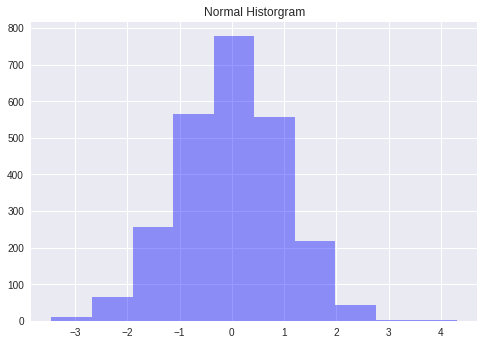
\includegraphics[width=0.8\textwidth]{./figs/normal-dist.png}
    \caption{$X \sim \mathcal{N}(0,\, 1)$ mit 2500 Samples}
    \label{fig:normal_dist}
\end{figure}

Ein weiterer Bestandteil von Schicht 1 sind \textit{Bijectors}. Bijectors bilden eine Zahl aus $\mathbb{R}^n$ auf $\mathbb{R}^m$ ab oder jeweils einer Submenge dieser. Aufgrund der im Bijector hinterlegten bijektiven Funktion ist dieser Schritt umkehrbar, daher: $x = f^{-1}(f(x))$. Dies ist besonders bei der Transformierung von Stichproben aus Verteilungen nützlich und wird folglich für das Erstellen von Modellen (Abschnitt \ref{sec:layer2}) und Berechnungen probabilistischer Interferenzen (Abschnitt \ref{sec:layer3}) eingesetzt. TFP bietet bereits einige vorgefertigte Bijectors unter \textbf{tfp.bijectors}\footnote{\url{https://www.tensorflow.org/probability/api_docs/python/tfp/bijectors}} an. 


\subsection{Schicht 2: Model Building}
\label{sec:layer2}
% TODO: Edward2
Edward2 / Probabilistic Layers with Keras / Trainable Distributions

In Abschnitt \ref{sec:example_air_quality} wird die Verwendung und probabilistischen Layers mit Keras anhand eines Beispiels verdeutlicht.

\subsection{Schicht 3: Probabilistic Inference}
\label{sec:layer3}
Als letzte Schicht enthält TFP Werkzeuge für probabilistische Inferenz. Dazu gehören \textit{Marcov chain Monte Carlo (MCMC)} Algorithmen, \textit{Variational Inference} Algorithmen und stochastische Optimierungsverfahren. 
Durch Sampling ermöglicht MCMC das Berechnen statistischer Modelle mit einer hohen Anzahl an Parametern. Eine analytische Herangehensweise ist bereits ab wenigen Parametern nicht mehr sinnvoll, da hierzu das Berechnen eines multidimensionalen Integrals erforderlich wäre. TFP bietet mehrere MCMC Algorithmen unter \textbf{tfp.mcmc} an. 

Listing \ref{lst:mcmc} zeigt einen Ausschnitt der Verwendung des Hamiltonian Monte Carlo Algorithmus. Die hier nicht gezeigte Auswertung würde in einer approximierten Verteilung des Parameters \textit{tau} für das gegebene Modell \textit{\_data\_model} resultieren. Ein praxisbezogenes und ausführlicheres Beispiel ist unter \url{https://github.com/tom-schoener/ml-probability/blob/master/tfp-evaluation/notebooks/mcmc.ipynb} einsehbar.

\begin{lstlisting}[language=Python, caption={Verwendung des Hamiltonian Monte Carlo Algorithmus (gekürzt)}, label={lst:mcmc}]
# Set the chain's start state.
initial_chain_state = [ 0.5 * tf.ones([], dtype=tf.float32, name="init_tau") ]

def joint_log_prob(_data_model, tau):
  rv_tau = tfd.Uniform()
  rv_observation = tfd.Poisson(rate=rv_tau)

  return rv_tau.log_prob(tau) + tf.reduce_sum(rv_observation.log_prob(_data_model))

# setup the chain
[ tau ], kernel_results = tfp.mcmc.sample_chain(
  num_results=1000,
  num_burnin_steps=500,
  current_state=initial_chain_state,
  kernel=tfp.mcmc.TransformedTransitionKernel(
    inner_kernel=tfp.mcmc.HamiltonianMonteCarlo(
      target_log_prob_fn=lambda tau: joint_log_prob(_data_model, tau)),
    bijector=[ tfp.bijectors.Sigmoid() ] # Maps [0,1] to R  
  )
)
\end{lstlisting}

Die in der API verwendeten Bezeichnungen decken sich hier größtenteils mit der in der Literatur verwendeten Sprache, wodurch die Übertragung von Konzepten aus unterschiedlichen Quellen deutlich vereinfacht wird. 

% TODO VI und Optimierungsverfahren kurz erklären

\section{Pragmatik und Semantik}

\section{Integration in Tensorflow}

\section{Anwendungsgebiete}

\section{Beispiel: Korrelation von Luftverschmutzung und Temperatur}
\label{sec:example_air_quality}

Das Jupyter Notebook für das folgende Beispiel ist unter \url{https://github.com/tom-schoener/ml-probability/blob/master/tfp-evaluation/notebooks/air_quality.ipynb} einsehbar.



\section{Fazit}


%----------------------------------------------------------------------------------------
%	Bibliography
%----------------------------------------------------------------------------------------
\newpage

\typeout{===== Section: literature}
%\bibliography{bibs/bibs}


\end{document}


